\chapter{Sestavení a testování}

Finální fází vývoje je kompletace jednotlivých částí. Pro řídicí jednotku byla zvolena univerzální montážní krabice s~vnějšími rozměry 217x138x\qty{82.2}{mm}. Do čelní strany krabice byly následně vyřezány otvory pro síťové zásuvky, napájecí konektor a konektory D-sub pro připojení periferí. Také byly vyvrtány otvory odkrývající jednotlivé stavové diody. Byly zvoleny zásuvky přímo určené k~montáži do panelu, navíc jsou vybaveny odklápěcím krytem a těsněním. Díky tomu jsou vhodným kandidátem pro použití v~systému řízení akvária. K~propojení silových vodičů uvnitř šasi bylo použito několik bezšroubových svorkovnic firmy Wago. Tyto svorkovnice jsou již samy o~sobě velmi spolehlivé, i přesto byly pro jistotu zajištěny proti otevřením izolační páskou. 

\begin{figure}[h!]
    \centering
    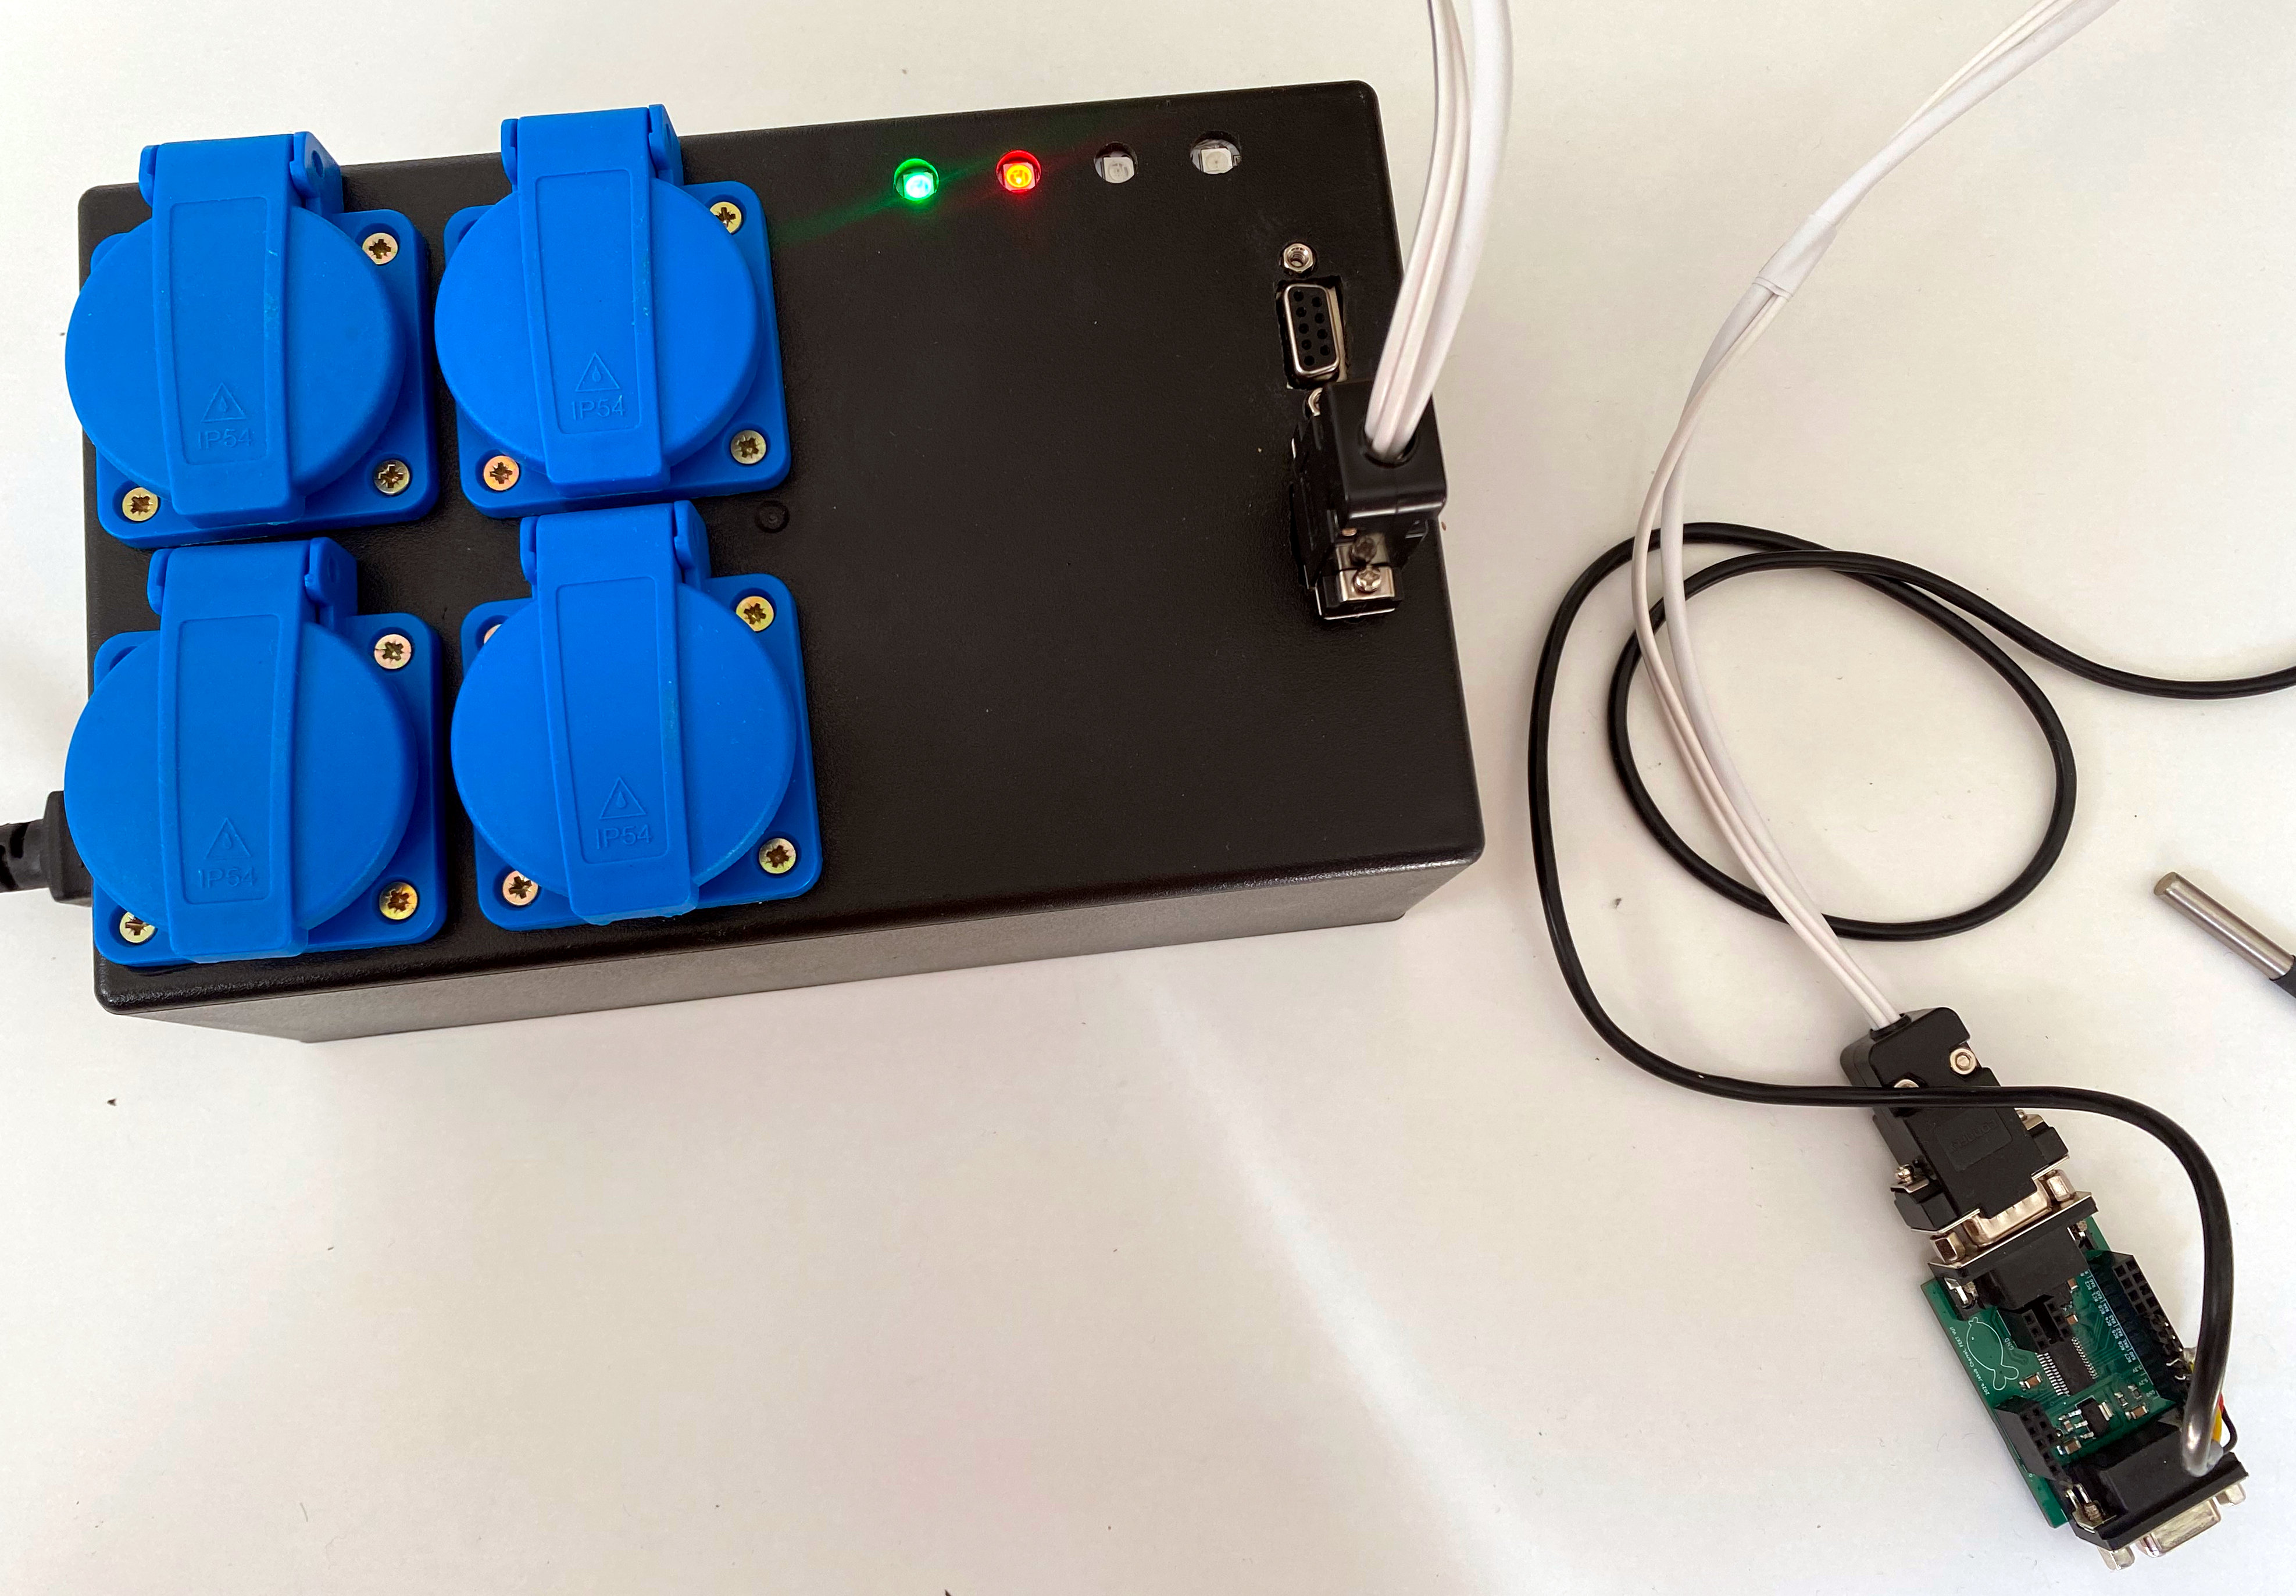
\includegraphics[width=0.8\textwidth]{obrazky/foto/zarizeni_beh.jpeg}
    \caption{Foto šasi řídicí jednotky v~běhu.}
    \label{fig:obrazky-foto-zarizeni_beh-jpeg}
\end{figure}

Modul externího napájecího zdroje \qty{24}{V} a modul relé jsou pevně připevněny ke stěnám resp. víku krabice. Při návrhu DPS řídicí jednotky byly záměrně zvoleny konektory určené k~montáži do panelu, při finálním sestavení zařízení však bylo zjištěno, že tloušťka stěny krabice je příliš velká a konektory takto uchyceny být nemohou. V~tuto chvíli je tedy DPS upevněna pouze provizorně. Možných řešení tohoto problému je několik, jako nejelegantnější se jeví použití metody 3D tisku. Do pravé části šasi bude vyřezán větší otvor, který bude celý překryt vytištěným panelem. Navržený panel pak bude disponovat vhodnějšími otvory pro uchycení konektorů D-sub, bude nabízet prostor pro již instalovaný LED pásek a také pro displej, který je plánovaným rozšířením zařízení.  

\begin{figure}[h!]
    \centering
    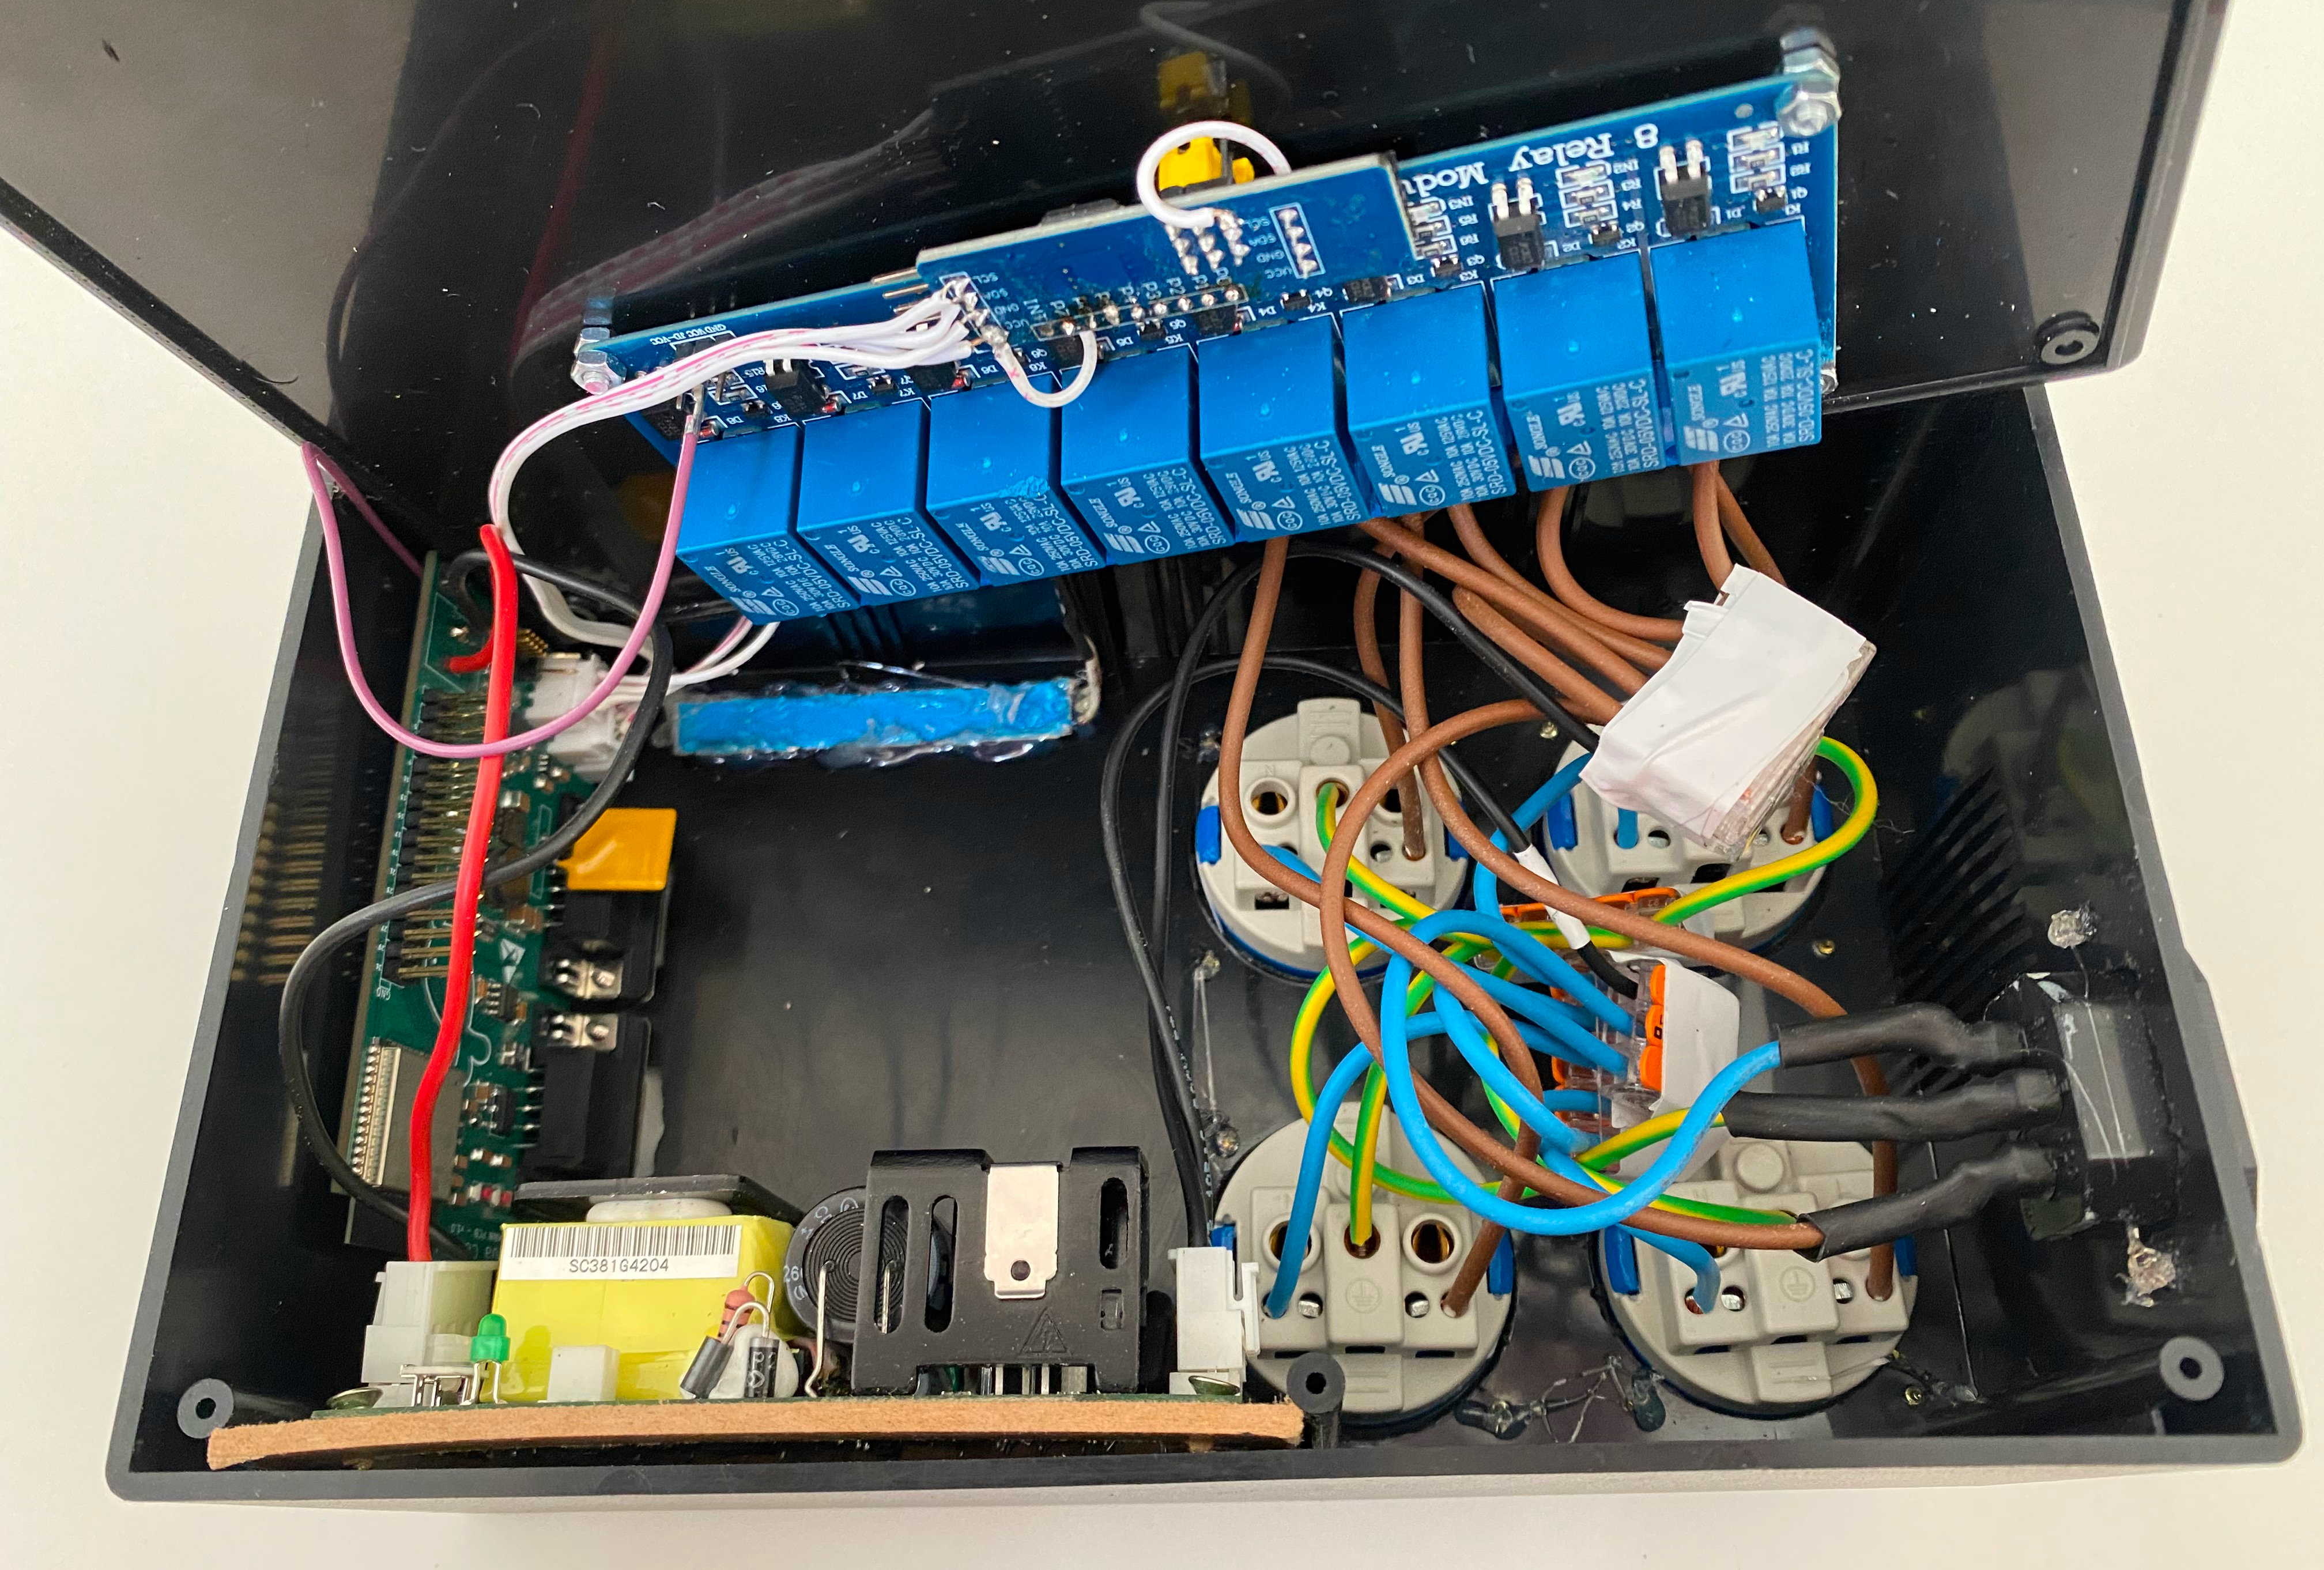
\includegraphics[width=0.8\textwidth]{obrazky/foto/ulozeni.jpeg}
    \caption{Pohled dovnitř šasi řídicí jednotky.}
    \label{fig:obrazky-foto-ulozeni-jpeg}
\end{figure}


Výsledný vzhled zařízení je zachycen na obr.~\ref{fig:obrazky-foto-zarizeni_beh-jpeg}, pohled dovnitř šasi řídicí jednotky je pak možný na obr.~\ref{fig:obrazky-foto-ulozeni-jpeg}.

\section{Testování a nalezené chyby}
    Vývoj a prvotní testy zařízení probíhaly mimo samotné šasi. Namísto externího napájecího modulu byl využíván laboratorní zdroj a řídicí jednotka i moduly periferií byly rozloženy na stole, aby byly snadno dostupné pro programování. V~této konfiguraci byla testována funkce jednotlivých modulů připojených jak samostatně, tak i společně ve stejnou dobu. Systém byl od počátku navrhován tak, aby veškerá konfigurace systému bylo prováděna přes webové rozhraní. Toto rozhodnutí mírně komplikovalo samotné testování funkce zařízení. Před samotným testováním totiž musela být vyvinuta alespoň provizorní webová aplikace a naprogramována spolehlivá komunikace se serverem. Tyto kroky pak zabraly mnohem více času, než byl původní předpoklad. V~průběhu vývoje bylo také postupně objeveno několik různě závažných návrhových chyb týkajících se hardwaru. 
    
    Nejvíce problémů se týká modulu LED osvětlení. Při návrhu byl položen špatný předpoklad pro minimální napětí LED pásků. Při napětí vypočteném v~rovnici~\ref{rovnice:led_modul} LED diody stále docela výrazně svítí a pro jejich plné zhasnutí je potřeba napětí přibližně o~\qty{1}{V} nižší. Tento problém je snadno řešitelný výměnou jednoho z~rezistorů děliče. Dalším problémem byl špatně zvolený pin mikrokontroléru. Periferie DAC jako jediná neumožňuje nastavení vlastního výstupního pinu a je pevně vázaná na dva konkrétní piny, musela tedy být zavedena drátová propojka. Jeden ze dvou navržených měničů nefunguje vůbec a příčina tohoto problému prozatím nebyla odhalena, je tedy možné využít pouze jeden kanál svícení. 

    Poslední problém se vyskytl až při montáži řídicí jednotky do krabice. Při nahrazení laboratorního zdroje externím modulem nastává problém se startem procesoru řídicí jednotky. Procesor se nezapne korektně a je potřeba stisknout resetovací tlačítko, pak již vše funguje jak má. Na vině je pravděpodobně jiná doba náběhu napájení, která má za následek nedodržení časování popsaného v~kapitole~\ref{sec:ridici-jendotka-esp32-modul}. 

    Dokud nebudou všechny tyto problémy odstraněny a zařízení dostatečně otestováno v~simulovaných podmínkách, nebylo by vhodné provádět test za reálného provozu. Akvarijní ryby by byly vystaveny nechtěnému stresu nebo by v~horším případě některá důležitá část systému vypověděla funkci. 

\section{Návrh budoucích vylepšení}
    Ačkoliv se za výrobkem skrývá velká spousta práce, ne všechny stanovené cíle byly dosaženy. V~tuto chvíli se jedná o~prototyp, který demonstruje funkci a možnosti zařízení, ne však zcela bezchybně. Ze zmíněných požadavků např. nebyla implementována možnost vzdálené aktualizace firmwaru. Samotné stažení firmwaru by v~tuto chvíli nebyl problém, jelikož komunikace se serverem je  implementována poměrně dobře. Je však potřeba zajistit, aby aktualizací nebyla narušena kompatibilita s~připojenými periferiemi nebo konfigurací získanou ze serveru. Pro spolehlivou implementaci této funkce tak bude potřeba daleko více času. Co se týče řídicí jednotky, je v~plánu vybavit ji také malým displejem, který může nést více informací než stavové diody. Např. by bylo užitečné znát počet detekovaných periferií a informovat uživatele o~úspěšném připojení nového modulu. 

    Díky modulární architektuře bude poměrně jednoduché systém rozšířit o~spoustu dalších funkcí, které se ukáží jako potřebné. Vizí blízké budoucnosti je dokončení sensoru pH a automatického krmítka.